\chapter{Desenvolvimento do projeto}
\label{chap:metod}
Nesta seção será descrito o procedimento utilizado para construção de cada um dos desafios.

\section{Webots}
O robô utilizado foi o Pionner o qual usa seus 16 sensores de distância pré-instalados para obter informações do mundo em todas as direções 
e um sensor adcional:o sensor de luminosidade que rastreia a irradiância local e envia um sinal para o robô quando ele lê mais de 750 W / m2, 
o que significa que está perto o suficiente da luminária de chão para disparar o STOP.

\subsection{controle}
A navegação do robô pelo mapa é baseada em uma máquina de 4 estados que determina se ele deve se mover para frente,
virar à esquerda, direita ou parar quando atingir seu objetivo final.

Assim, a divisão foi feita em quatro casos, são eles:
\begin{itemize}
    \item FORWARD: Anda para frente e se houver algum obstáculo à frente ele começa a tomar a decisão de virar em qualquer direção para evitá-lo.
    \item ESQUERDA: Vire à esquerda até que a detecção de objetos não seja mais possível;
    \item DIREITA: Vire à direita até que a detecção de objetos não seja mais possível;
    \item STOP: Quando o sensor de luz detecta a quantidade de luminosidade configurada (neste caso 750 W / m2), o robô deve parar.
\end{itemize}
Todos os sensores de distância coletam dados do ambiente que determinam se o robô deve se mover para frente ou para os lados.
\section{Turtlesim}
Para que o desafio seja cumprido é necessário rodar o roscore e o nó para que a janela da turtle apareça na tela.

\begin{figure} [h!]	
    \centering
    \caption{inicializando o ros}
    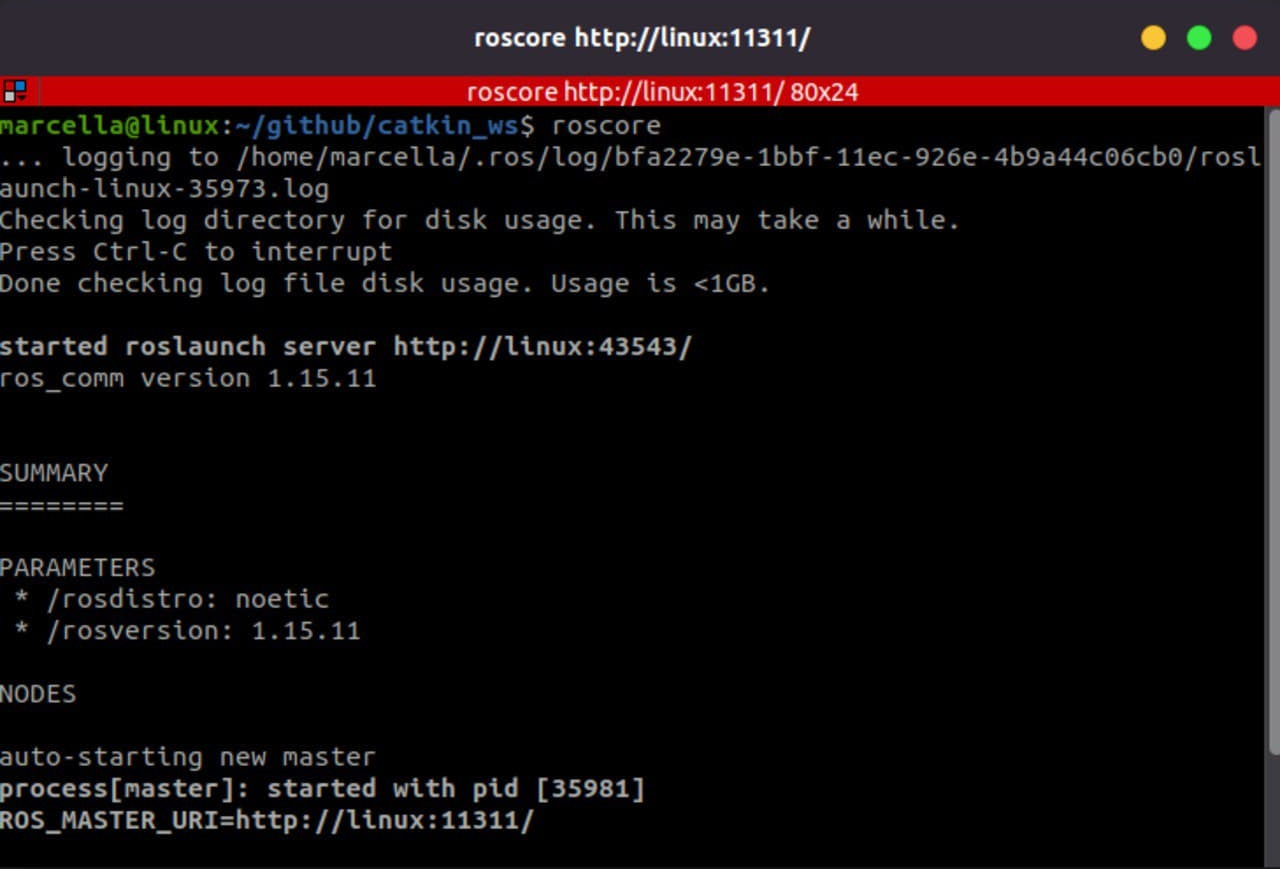
\includegraphics[width=0.5\textwidth]{roscore.jpg}
    \caption*{Fonte: Autoria própria.}
    \label{fig:roscore}
\end{figure}

\begin{figure} [h!]	
    \centering
    \caption{ Rodando o nó do turtlesim}
    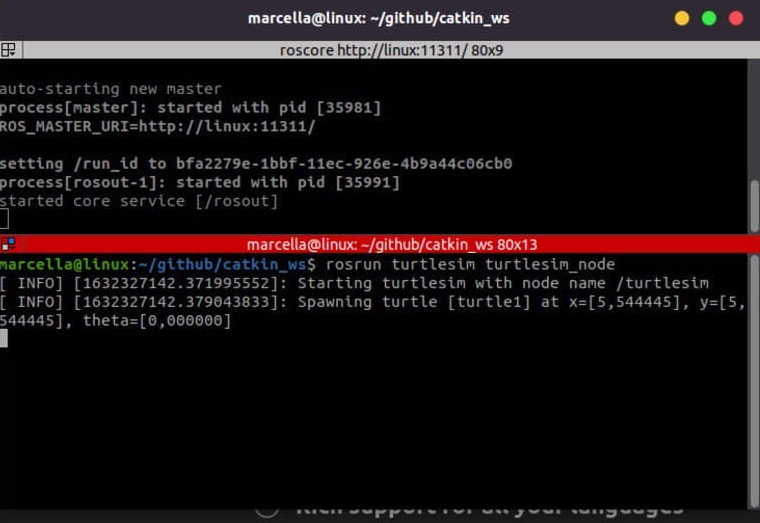
\includegraphics[width=0.5\textwidth]{rosrum.jpg}
    \caption*{Fonte: Autoria própria.}
    \label{fig:rosrum}
\end{figure}
por fim executa-se o arquivo .py quue foi a liguagem escolhida para completar este desafio, como mostra a figura abaixo.
\begin{figure} [h!]	
    \centering
    \caption{ Executando arquivo}
    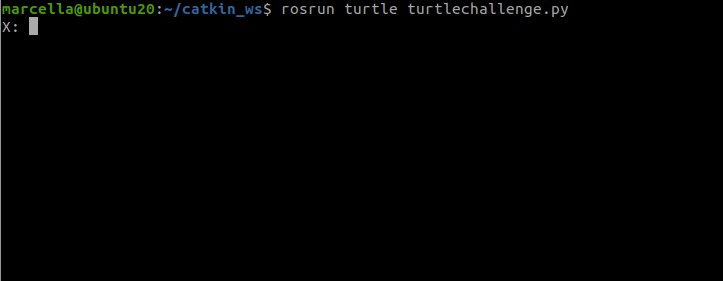
\includegraphics[width=0.5\textwidth]{xey.jpeg}
    \caption*{Fonte: Autoria própria.}
    \label{fig:excute.py}
\end{figure}
É posto as coordenadas x e y no caso do exemplo do desafio é 1 e 1 e a tartaruga deve ir até essa coordenada quando o erro for no máximo 0.1.
\section{Husky}
\subsection{Move Base}
Após toda a configuração e instalação dos pacotes do Husky encontrado no repositório https://github.com/husky/husky, foi executado o nó move-base no qual será enviado um comando para o robô Husky que tentará atingir a posição enviada desviando dos obstáculos e caso entre em alguma posição em que se esteja travado executa comportamentos de recuperação para continuar o trajeto enviado.

Para a execução do nó move-base é necessário trés comandos o primeiro inicia o ambiente de simulação o gazebo, o segundo o visualizador rviz e o terceiro a demonstração move-base.
\begin{figure} [h!]	
    \centering
    \caption{Comandos move base}
    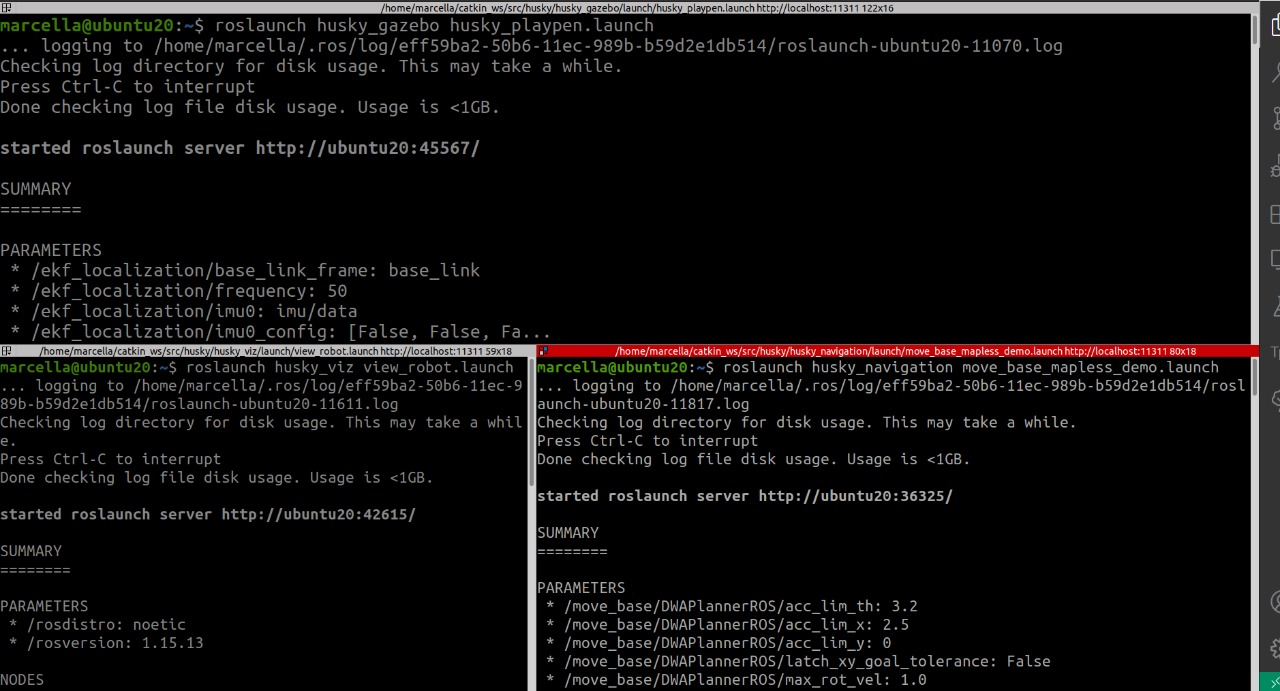
\includegraphics[width=1.0\textwidth]{comandosmb.jpeg}
    \caption*{Fonte: Autoria própria.}
    \label{fig:movebase}
\end{figure}
\subsection{AMCL}
O Tutorial amcl do Husky mostra como é usado o move-base com o sendo assim, amcl obtém um mapa baseado em laser que precisa ser ativado no description do robô encontrado no próprio repositório após a ativação o laser faz varreduras e transforma em mensagens que geram estimativas de posição.
\begin{figure} [h!]	
    \centering
    \caption{Comandos amcl}
    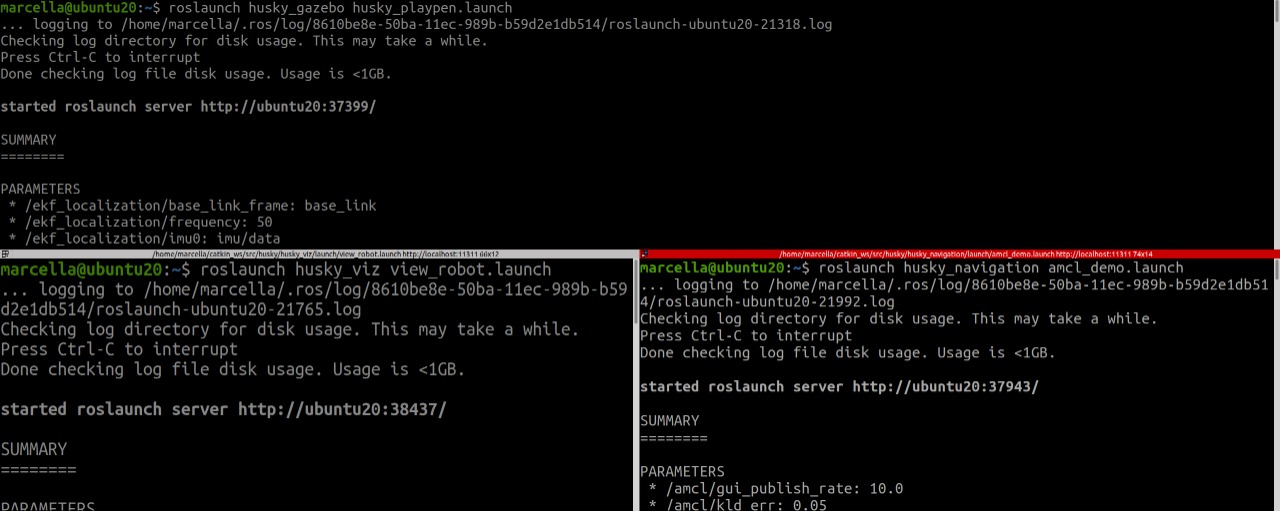
\includegraphics[width=0.9\textwidth]{comandosamcl.jpeg}
    \caption*{Fonte: Autoria própria.}
    \label{fig:amcl}
\end{figure} 
\subsection{gmapping}
Após a execução do nó slam-gmapping será levado para o tópico sensor-msgs/LaserScan mensagens e constrói um mapa a partir dos dados de laser e posições coletados pelo husky.
\begin{figure} [h!]	
    \centering
    \caption{Comandos gmapping}
    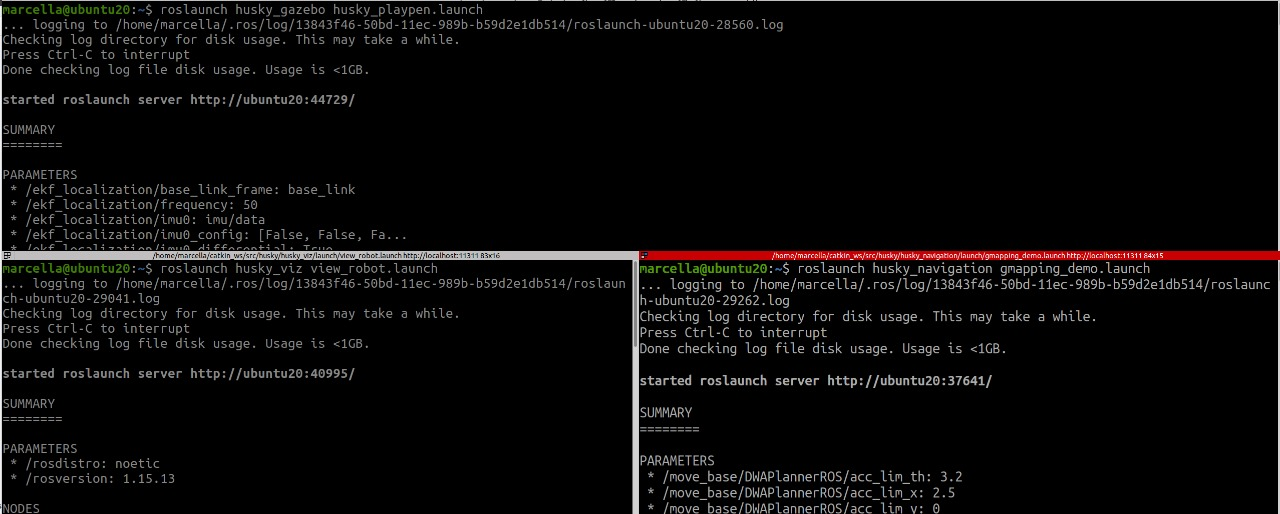
\includegraphics[width=0.9\textwidth]{comandogm.jpeg}
    \caption*{Fonte: Autoria própria.}
    \label{fig:gmapping}
\end{figure}
\subsection{Frontier-exploration}
O Frontier-exploration pacote fornece um costmap-2d que fornece uma implementação de um mapa de custo 2D que leva em dados de sensor do mundo, constrói uma grade de ocupação 2D ou 3D dos dados, e actionlib cliente que fornece uma interface padronizada com tarefas preemptivas
\begin{figure} [h!]	
    \centering
    \caption{Comandos frontier-exploration }
    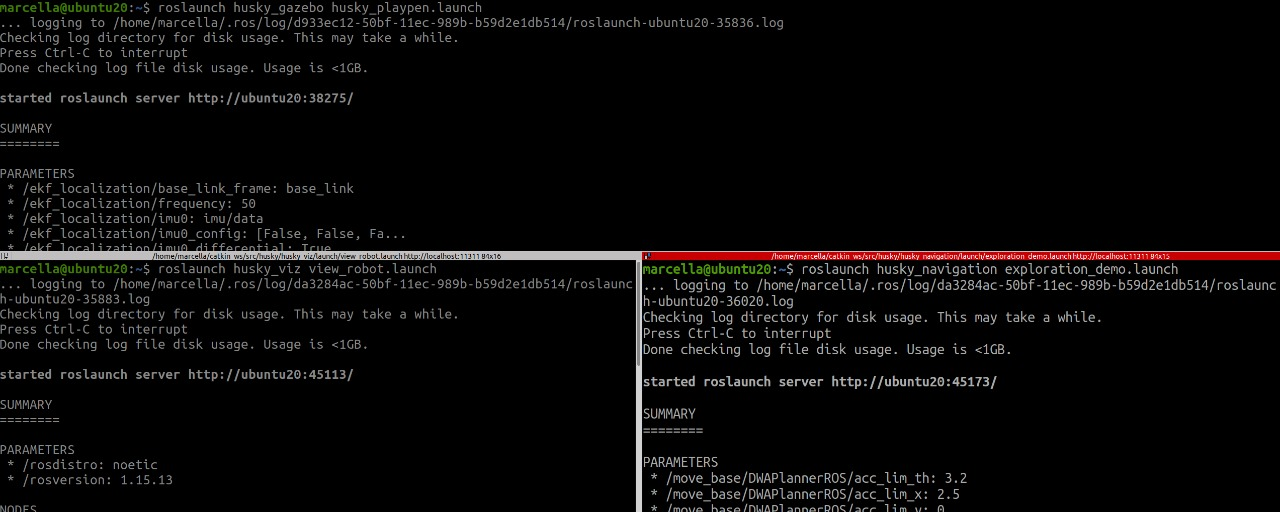
\includegraphics[width=1.0\textwidth]{comandosf.jpeg}
    \caption*{Fonte: Autoria própria.}
    \label{fig:frontier-exploration}
\end{figure}
\section{CPP}
Após assistir os tutoriais de CPP e obter os conhecimentos necessários foi possível resolver os desafios propostos no workbook de c++ os Desafios foram: 

    -Triângulo de Pascal que consiste em um programa para calcular o valor de uma determinada posição no Triângulo de Pascal.

    A maneira de calcular o valor de qualquer posição é somar os números à direita e à esquerda da posição na linha anterior.

   O programa solicita que o usuário insira uma linha e assim é dado o valor correspondente.

   Por exemplo, para calcular o número do meio na terceira linha, você adiciona 1 e 1; os lados do triângulo são sempre 1 porque você só adiciona o número à esquerda superior ou à direita superior, o exemplo pode ser melhor visualizado na figura abaixo.

\begin{figure} [h!]	
    \centering
    \caption{triangulo de pascal}
    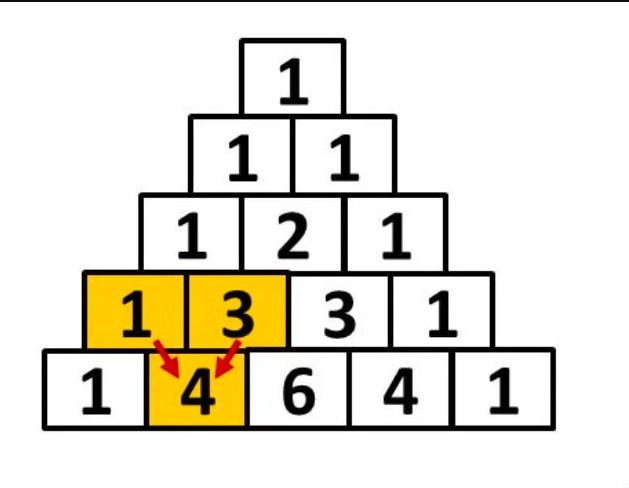
\includegraphics[width=0.4\textwidth]{triangulodepascal.jpeg}
    \caption*{Fonte:https://www.todamateria.com.br/triangulo-de-pascal/}
    \label{fig:triangulodepascal}
\end{figure}


    -Desafio da Permutação de Cordas que se trata de um programa para exibir todas as permutações possíveis de uma determinada string de entrada.se a string contém caracteres duplicados, pode ter vários resultados repetidos.A saida deve ser dada uma palavra por linha.

\begin{figure} [h!]	
    \centering
    \caption{Permutação}
    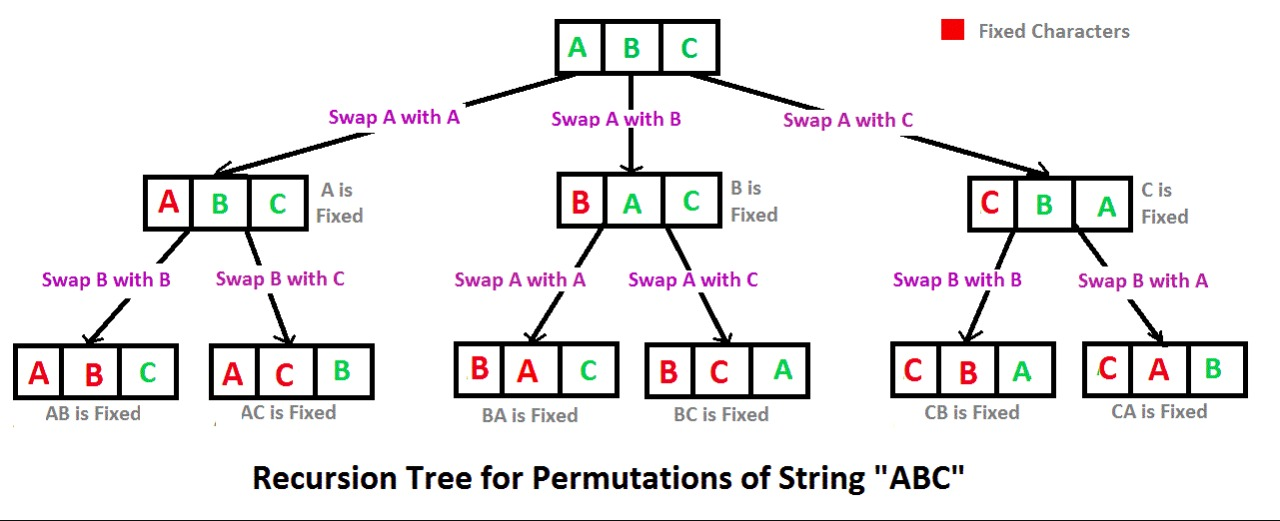
\includegraphics[width=0.6\textwidth]{permutacao.jpeg}
    \caption*{Fonte:https://i.stack.imgur.com/8DK5W.gif}
    \label{fig:permutacaodeletras}
\end{figure}

-Programa de Autoimpressão que é um programa que, quando executado, imprimirá seu código-fonte. Este código-fonte, por sua vez, deve compilar e imprimir a si mesmo. 

\begin{figure} [h!]	
    \centering
    \caption{Permutação}
    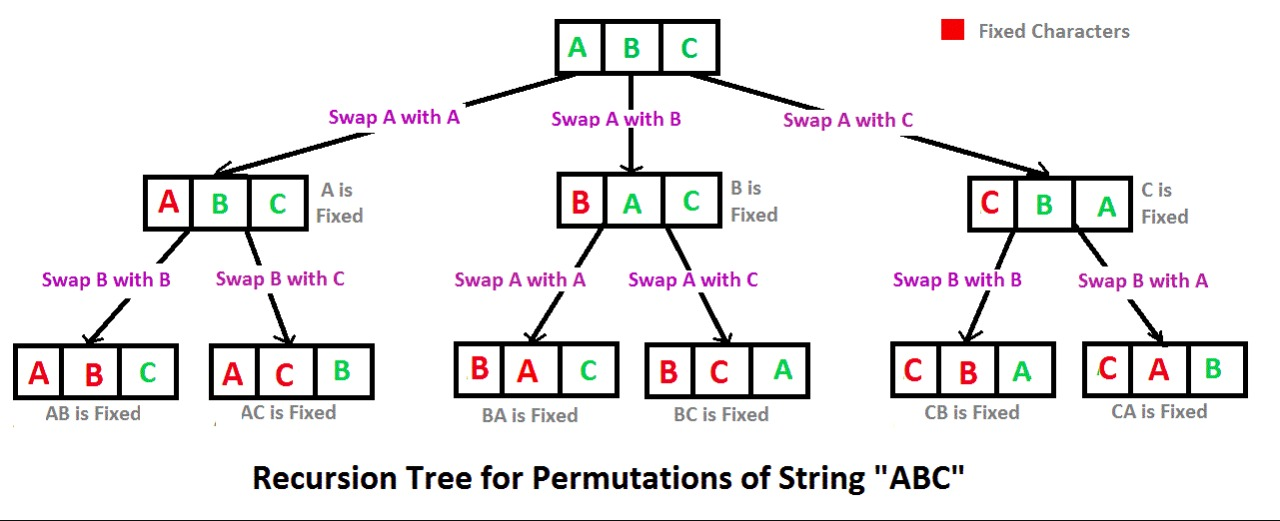
\includegraphics[width=0.6\textwidth]{permutacao.jpeg}
    \caption*{Fonte:https://i.stack.imgur.com/8DK5W.gif}
    \label{fig:permutacaodeletras}
\end{figure}
\section{Python}
Após assistir os tutoriais de Python e obter os conhecimentos necessários foi possível resolver os desafios propostos nos workbooks 1 e 2 de python começando pelo 1 e os desafios foram: 

-Mediana de Três Valores: que consiste em uma função que recebe três números como parâmetros e retorna o valor médio desses parâmetros como seu resultado.

-Os Doze Dias do Natal: É uma canção repetitiva que descreve uma lista cada vez mais longa de presentes enviados ao verdadeiro amor de cada um em cada um dos 12 dias. Um único presente é enviado no primeiro dia. Um novo presente é adicionado à coleção em cada dia adicional e, em seguida e assim por diante.
O programa exibe a letra completa da musica.

-Centralize uma corda no terminal: Contém uma função que tenha uma string como seu primeiro parâmetro e a largura do terminal como seu segundo parâmetro e retorna uma nova string que consiste na string original e o número correto de espaços iniciais para que a string original apareça centralizada dentro da largura fornecida quando for impressa.

-Capitalize-o: Como muitas pessoas não usam letras maiúsculas corretamente, especialmente ao digitar em pequenos dispositivos como smartphones. Neste desafio a função coloca em maiúscula os caracteres apropriados em uma string e o programa principal printa o texto correto.

-Uma string representa um inteiro: A função chamada isInteger determina se os caracteres em uma string representam ou não um inteiro válido.

-É um número primo? Um número primo é um número inteiro maior que 1 que só é divisível por um e por ele mesmo. A função determina se o numero colocado é primo ou não, retornando é primo se for, e não primo caso contrário. 

-Senha aleatória: A função gera uma senha aleatória pela biblioteca random. A senha deve ter um comprimento aleatório de 7 a 10 caracteres, cada caractere foi selecionado aleatoriamente das posições 33 a 126 na tabela ASCII. O programa printa a senha gerada aleatoriamente como seu único resultado.

-Verifique uma senha: A função que determina se uma senha é válida ou não e retorna senha ok se a senha passada for válida.

-Conversões de base arbitrária: O programa permite ao usuário converter um número de uma base para outra, oferecendo suporte a bases entre 2 e 16, tanto para o número de entrada quanto para o número de resultado. Se o usuário escolher uma base fora dessa faixa, uma mensagem de erro apropriada deve ser exibida e o programa deve ser encerrado.

-Reduzir uma fração aos termos mais baixos: A função que recebe dois inteiros positivos que representam o numerador e o denominador e reduz a menor fração possível usando a função reduceFractions. 

-Reduzir Medidas: A função que expresse um volume usando as maiores unidades possíveis, tem o número de unidades como seu primeiro parâmetro e a unidade de medida (xícara, colher de sopa ou colher de chá) como seu segundo parâmetro e retorna uma string representando a medida como resultado da função. 

-Datas mágicas: Uma data mágica é uma data em que o dia multiplicado pelo mês é igual ao ano de dois dígitos. A função determina se uma data é ou não uma data mágica. 

Logo após o termino do workbook 1 foi inciada a resolução do workbook 2 que consiste nos seguintes desafios:

-Cifra de César: Cada letra na mensagem original é deslocada em 3 lugares. Como resultado, A torna-se D, B torna-se E, C torna-se F, D torna-se G, etc. As últimas três letras do alfabeto são agrupadas desde o início: X torna-se A, Y torna-se B e Z torna-se C. 
O  programa implementa uma cifra de César, o usuário fornece a mensagem e o valor do turno e, em seguida, exibe a mensagem alterada e contém deslocamento negativo para que possa ser usado para codificar e decodificar mensagens.

-Verifique uma senha: A função determina se uma senha é válida ou não. Definiremos uma boa senha como aquela que tem pelo menos 8 caracteres e contém pelo menos uma letra maiúscula, pelo menos uma letra minúscula e pelo menos um número. Retorna senha ok se a senha passada for válida, caso contrário, retorna digite outra senha. Inclui um programa principal que lê a senha do usuário e informa se ela é ou não válida.

-Números perfeitos: Um inteiro, n, é considerado perfeito quando a soma de todos os divisores próprios de n é igual a n. A função determina se um número inteiro positivo é perfeito ou não. Se for um número perfeito, sua função retornará verdadeiro. Caso contrário, ele retornará falso. Além disso, o programa identifica e exibi todos os números perfeitos entre 1 e 10.000.

-Palíndromo Recursivo: A função recursiva determina se uma string é ou não um palíndromo. Qualquer string mais longa é um palíndromo se seu primeiro e último caracteres coincidir e se a string formada pela remoção do primeiro e do último caracteres também for um palíndromo.
O programa ler uma string do usuário e exibe se é ou não um palíndromo.

% %--------- NEW SECTION ----------------------
% \section{Interface do Usuário}
% \label{sec:ui}
% \lipsum[1]

% %--------- NEW SECTION ----------------------
% \section{Simulação do sistema}
% \label{sec:sim}
% \lipsum[2-4]

